\documentclass[%
 reprint,
%superscriptaddress,
%groupedaddress,
%unsortedaddress,
%runinaddress,
%frontmatterverbose, 
%preprint,
%showpacs,preprintnumbers,
%nofootinbib,
%nobibnotes,
%bibnotes,
 amsmath,amssymb,
 aps,
%pra,
%prb,
%rmp,
%prstab,
%prstper,
%floatfix,
]{revtex4-1}

\usepackage{graphicx}% Include figure files
\usepackage{dcolumn}% Align table columns on decimal point
\usepackage{bm}% bold math

\begin{document}

\title{First Exclusive Measurement of Deep Virtual Compton Scattering off $^4$He: Toward the 3D tomography of nuclei}

\author{M. Hattawy, ...}
\affiliation{...}
\author{R. Dupr\'e}
\affiliation{Institut de Physique Nucl\'eaire d'Orsay, CNRS-IN2P3,\\ 
Universit\'e Paris-Sud, Universit\'e Paris-Saclay, 91406 Orsay, France.}

\date{\today}

\begin{abstract}
We report the first exclusive measurement of deeply virtual Compton scattering 
(DVCS) off a nuclei with the CLAS detector at the Jefferson laboratory. The 
observed beam spin asymmetries are significantly larger than for proton, 
confirming expectations from calculations using the plane wave impulse 
approximation. We present an 
extraction of the single generalized parton distribution (GPD) of the spin-0 
helium-4 nuclei in a completely model independent way. This result demonstrate the 
strength of the method and opens a new and unique access into the partonic structure 
of nuclei.
\end{abstract}

\pacs{Valid PACS appear here}

\maketitle

%\section{Introduction}
% Now many letters do not put any sections. Maybe we should consider doing the same

The generalized parton distribution (GPD) framework developped in the past 
two decades~\cite{}
offers a unique access into hadron 3D structure through deeply virtual Compton
scattering (DVCS), depicted in figure~\ref{fig:DVCS}, and other exclusive 
processes. Many measurements on the proton
at several energies have now be reported~\cite{} and phenomenological work
have demonstrated the solidity of the method to extract the tomography of the
nucleon from these data~\cite{}. 

\begin{figure}[htbp]
\caption{\label{fig:DVCS} Diagram for the coherent DVCS in the plane wave approximation.}
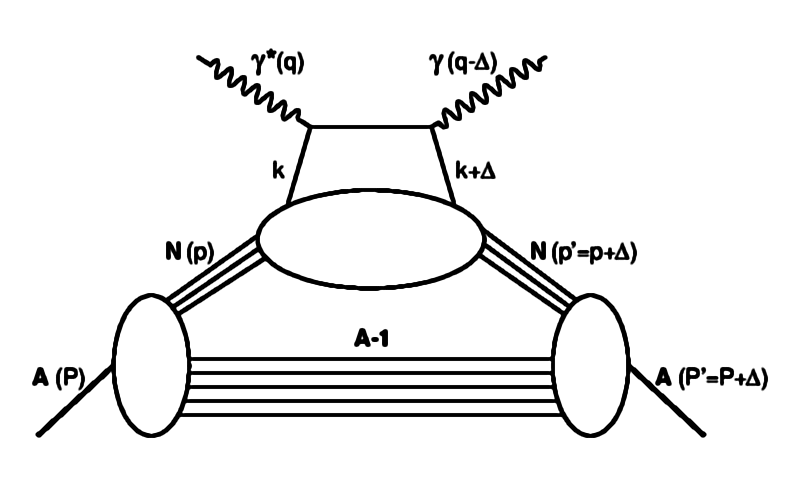
\includegraphics[width=8.6cm]{DVCS.png}
\end{figure}

At the same time, the partonic structure of nuclei has remained a mystery
for the past three decades, as we are still unable to explain properly the 
infamous EMC effect~\cite{}. First observed in 1983 by the EMC 
collaboration, it describes the difference between the partonic structure of
free and bound nucleons. Understanding the source of this difference remains 
today a topic of active research~\cite{},
questionning the basics of our understanding of nuclei and their 
structure~\cite{}. Studies based on inclusive measurements of the
effect provide a very detailed description~\cite{} but 
are still unable to tackle the question definitively. Therefore,
using the GPD framework and exclusive channels to study the nuclei in three 
dimensions will give completely new information that will affect our understanding
of the EMC effect in an unprecedented way~\cite{}. 
%In particular, the GPDs 
%allow to isolate the components of the nuclei which are not nucleonic~\cite{}. 

The measurement of DVCS on helium-4 is in this regard the perfect experiment for
several reasons. First, Helium 4 is of spin-0, such that a single GPD ($H$) is
necessary for the description of the DVCS at leading order. This feature allows for a
completely model independant extraction of the CFF from data that is impossible for 
protons and neutrons which have 4 GPDs~\cite{}. Second, 
helium 4 is dense and experience 
already a significant EMC effect, while being simple enough that its nuclear
structure is well known~\cite{}. Third, being 
light enough helium-4 can exit
a light target and be experimentally measured in a coherent DVCS process, 
insuring the exclusivity of the 
measurement. This point is especially important because we are probing with a 
multi-GeV interaction a nuclei bound by only a few MeV, this leads in the 
overwhelming majority of the cases to the incoherent break-up of the target.
The HERMES collaboration has measured nuclear DVCS~\cite{} without the 
detection of the recoils separating the coherent and incoherent channels 
based on the measurement of the transfered 4-momentum $t$, leading
to controversy in the interpretation of their results~\cite{}.

%\section{Experiment}
We report here our exclusive measurement of coherent DVCS off helium-4 
at the Jefferson labortory
(JLab), while our results for the incoherent channel will be presented in
another paper. JLab delivers a nearly 100\% duty factor, 6~GeV linearly 
polarized electrons into three experimental halls. Our experiment ran for 3 
months in 2009 using the CEBAF Large Acceptance Spectrometer (CLAS) in 
Hall-B. This detector is large acceptance covering nearly 2$\pi$ and is 
composed of drift chambers, Cherenkov counters, scintillator counters and 
an electro-magnetic calorimeter. It allows to detect accurately electrons 
which provide the trigger for the experiment. It is complemented for DVCS 
experiments with an inner electro-magnetic calorimeter made of PbWO crystals 
to detect the photons emitted at low angle and with a solenoid to keep the 
Moller electrons produced along the beam line to get into our detectors.

In order to ensure the coherence of the process, we also detect the recoiling 
helium-4 nuclei. We built a small and light radial time projection chamber 
(RTPC) to detect recoiling helium nuclei down to energies of few MeVs. The 
chamber, shown in figure~\ref{fig:rtpc}, is surrounding the gaseous target 
filled with 6~atm helium-4 and is 20 cm long with a 3 cm radial drift 
length. The detector was specifically calibrated for helium-4 nuclei using 
elastic scattering produced with a 1.2~GeV electron beam.
To ensure that the process is exclusive, we apply cuts on 
several kinematic variables (figure~\ref{fig:exclu}) such as missing energy,
mass and momentum. The cuts are chosen to represent consistently 3 half width 
at half maximum in order to avoid any bias in the selection.

%\section{DVCS Events Selection}

\begin{figure}[tb!]
\caption{\label{fig:rtpc} A cross section of the RTPC taken on a plane perpendicular to the 
beam line, with a typical $^4He$ track crossing the drift volume.}
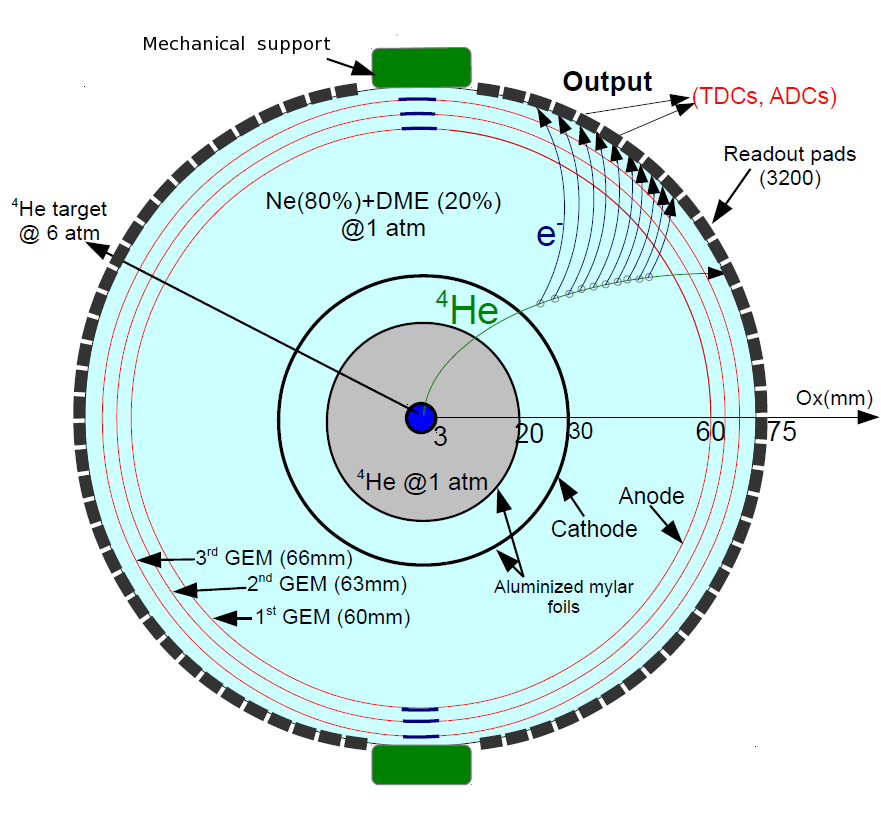
\includegraphics[width=7.4cm]{RTPC.png}
\end{figure}


\begin{figure*}[tb!]
\caption{\label{fig:exclu} The coherent DVCS exclusivity cuts. The blue 
distributions represent the coherent DVCS events candidate. The shaded 
distributions represent the events which passed all the exclusivity cuts 
except the quantity plotted. The vertical red lines represent $3\sigma$ cuts.}
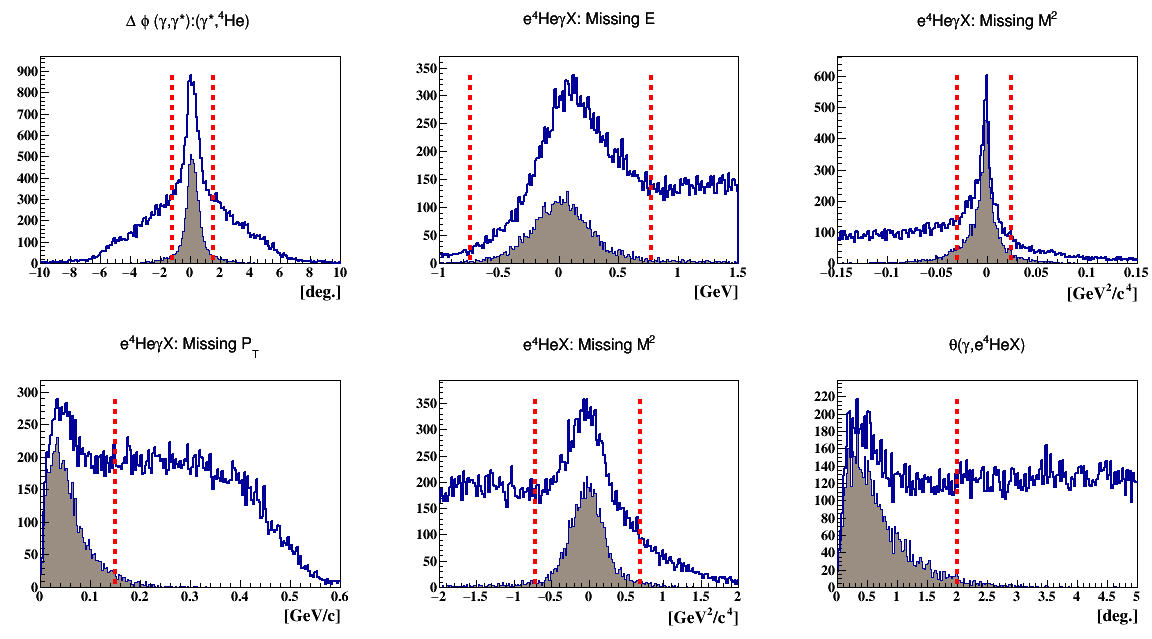
\includegraphics[width=16.0cm]{all_coh_exc_cuts.png}
\end{figure*}

We identified several background contributions to the DVCS process, in 
particular accidental events and exclusive deeply virtual 
$\pi^0$ production (DV$\pi^0$P). The accidental
events where the different particles come from different events are 
suppressed by the limited phase space allowed by the exclusivity cuts. We 
estimate the accidental events to represent 4.1\% of our sample. This relatively 
large number is due to the small cross section of the DVCS. We evaluated this contribution by
selecting events passing all our cuts but with particles originating from 
different verteces. 

Another important source of background is the deeply virtual 
$\pi^0$ production (DV$\pi^0$P), which can easily be mistaken
with DVCS when one of the two photons of the $\pi^0$ decay is produced at
low energy in the laboratory frame. To estimate the importance of
this background, we developped an event generator 
that we calibrated to match our measured experimental yield of exclusive 
$pi^0$. We used this generator together 
with a GEANT3 simulation of our detection system to estimate the ratio 
of acceptance between DV$\pi^0$P where the two photons are detected and those
where only one photon is detected and would pass our 
DVCS selection cuts. This ratio obtained from simulation is then multiplied by 
the measured yield of DV$\pi^0$P events, indicating a contamination of 2 to 4\%. 
The study of systematics errors showed that the main contributions come from 
the choice of the DVCS exclusivity cuts (8\%) and the large binning size 
(5.1\%). However added quadratically, these errors sum up to 10\% which remain 
for all bins well below the statistical errors.

%\section{Results}

We show the obtained assymetries after all corrections as a function of 
$\phi$ and $-t$ in figure~\ref{fig:assym}. The first observation is the
that the assymetries follow the expected sin($\phi$) dominated shape
and that the size of these assymetries at $90^\circ$ is much larger than the one
observed on proton targets~\cite{} (15-20\%). These results were expected from 
theory~\cite{} and demonstrate that we successfully isolated the coherent
DVCS channel.


\begin{figure*}[htbp]
\caption{\label{fig:assym} The coherent $A_{LU}$ as a function of $\phi$ in 
$-t$ bins. The error bars 
represent the statistical and the systematic uncertainties added 
quadratically, shown on top in green are error bars representing only the 
statistical uncertainties. The brown bands represent the systematic 
uncertainties, including the normalisation systematic uncertainties. The red 
curves represent fits in the form of equation \ref{eq:A_LU-coh}.}
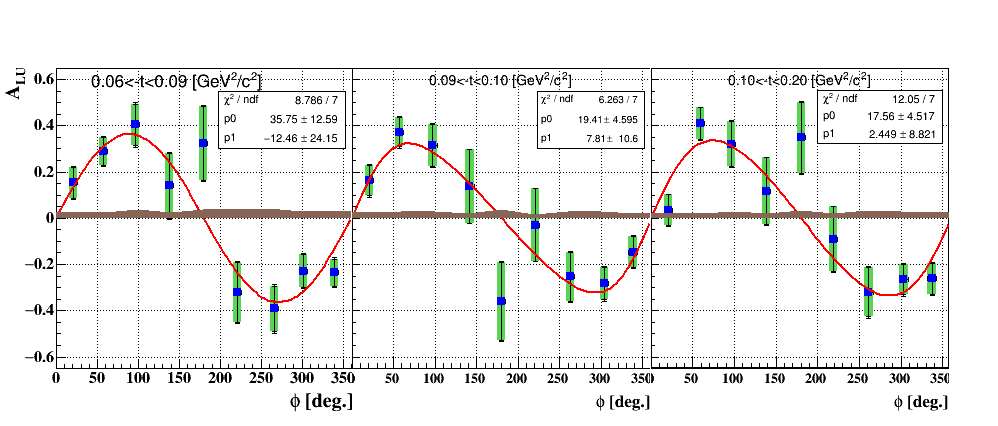
\includegraphics[width=14cm]{coh_alu_t_phi.png}
\end{figure*}


\begin{figure}[htbp]
\caption{\label{fig:CFF} The model-independent extraction of the imaginary (blue points) and 
real (red points) parts of the $^4$He CFF $\mathcal{H}_A$, as functions of 
$Q^{2}$ (on the top right), $x_B$ (on the top left), and $t$ (on the bottom).
NEED TO ADD GUZEY MODEL}
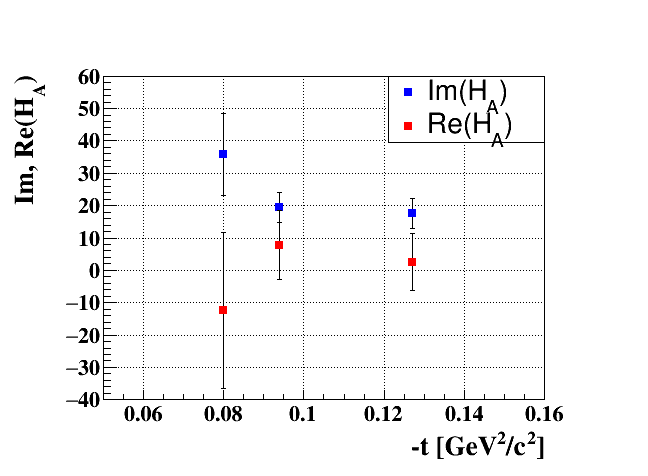
\includegraphics[width=8cm]{HA_t.png}
\end{figure}


As advertised above, we extract the GPD $H$ in a model independent way 
(figure~\ref{fig:CFF}). This is possible using the beam-spin asymmetry ($A_{LU}$) 
expression for spin-zero target at leading twist~\cite{BM_2009}:
\begin{equation}
\begin{split}
A_{LU}(\phi) &= \\
 \frac{\alpha_{0}(\phi) \, \Im m(\mathcal{H}_{A})}
{\alpha_{1}(\phi) + \alpha_{2}(\phi) \, \Re e(\mathcal{H}_{A}) + \alpha_{3}(\phi) \, 
\big( 
\Re e(\mathcal{H}_{A})^{2} + \Im m(\mathcal{H}_{A})^{2} \big)}
\label{eq:A_LU-coh}
\end{split}
\end{equation}
where $\Im m(\mathcal{H}_{A})$ and $\Re e(\mathcal{H}_{A})$ are the imaginary 
and real parts of the CFF $\mathcal{H}_{A}$ associated to the GPD $H_A$. The 
$\alpha_{i}$'s are $\phi$-dependent kinematical factors that depend on the 
nuclear form factor $F_A$ and the independent variables $Q^2$, $x_{B}$ and $t$.  
These factors are simplified as:
\begin{equation}
   \alpha_0 (\phi) =\frac{x_{A}(1+\epsilon^2)^2}{y} S{++}(1) \sin(\phi)\\
\end{equation}
\begin{equation}
    \alpha_1 (\phi) = c_0^{BH}+c_1^{BH} \cos({\phi})+c_2^{BH} \cos(2\phi)\\ 
\end{equation}
\begin{equation}
   \alpha_2 (\phi) = \frac{x_{A}(1+\epsilon^2)^2}{y}  \left( C_{++}(0) +  
C_{++}(1) cos(\phi) \right)\\
\end{equation}
\begin{equation}
\alpha_3 (\phi) = \frac{x^{2}_{A}t(1+\epsilon^2)^2}{y} {\mathcal P}_1(\phi) 
{\mathcal P}_2(\phi) \cdot 2 \frac{2-2y+y^2 + \frac{\epsilon^2}{2}y^2}{1 + 
\epsilon^2}
\end{equation}
Where $S{++}(1)$, $C_{++}(0)$, and $C_{++}(1)$ are the Fourier harmonics in the 
leptonic tensor. Their explicit expressions can be found in \cite{}.  

The result of this extraction shown in figure~\ref{fig:CFF} is very promising.
We first see that the imaginary part of $H$ comes out of the data with 
error bars comparable to the statistical error of data. For the real part,
the extraction appears to be more difficult, which is expected because 
$\alpha_2$ is suppressed compared to $\alpha_0$ contribution. However,
we note that the error bars are finite and that the fit converge without 
placing any bound on the CFF, which is necessary on proton targets.

%\section{Summary}

We presented the first exclusive measurement of coherent nuclear DVCS and the
first extraction of the CFF of the helium-4 nuclei. These
results, while limited by statistical precision, show a very strong signal 
in the beam spin assymetry and demonstrate the possibility to perform a
completely model independent extraction of the CFF even with large 
statistical uncertainties. This opens many new perspectives 
for the study of the structure of nuclei in terms of quarks and gluons
and pave the way for future more precise measurements at JLab 12~GeV
and possibly at an Electron-Ion Collider (EIC).

\section*{Acknowledgments}
Guzey and Liuti

\section*{Bibliography}
Biblio

\end{document}

